\documentclass{sig-alternate}
  \pdfpagewidth=8.5truein
  \pdfpageheight=11truein

\begin{document}
%
% --- Author Metadata here ---
\conferenceinfo{SAC'09}{March 8-12, 2009, Honolulu, Hawaii,
U.S.A.}
\CopyrightYear{2009} % Allows default copyright year (2002) to be over-ridden - IF NEED BE.
\crdata{978-1-60558-166-8/09/03}  % Allows default copyright data (X-XXXXX-XX-X/XX/XX) to be over-ridden.
% --- End of Author Metadata ---

\title{Web Semantization}
%\subtitle{Subtitle
%\titlenote{A full version of this paper is available as
%\textit{Author's Guide to Preparing ACM SIG Proceedings Using
%\LaTeX$2_\epsilon$\ and BibTeX} at
%\texttt{www.acm.org/eaddress.htm}}}
%
% You need the command \numberofauthors to handle the "boxing"
% and alignment of the authors under the title, and to add
% a section for authors number 4 through n.
%
% Up to the first three authors are aligned under the title;
% use the \alignauthor commands below to handle those names
% and affiliations. Add names, affiliations, addresses for
% additional authors as the argument to \additionalauthors;
% these will be set for you without further effort on your
% part as the last section in the body of your article BEFORE
% References or any Appendices.

\numberofauthors{4}
%
% You can go ahead and credit authors number 4+ here;
% their names will appear in a section called
% "Additional Authors" just before the Appendices
% (if there are any) or Bibliography (if there
% aren't)

% Put no more than the first THREE authors in the \author command
\author{
%
% The command \alignauthor (no curly braces needed) should
% precede each author name, affiliation/snail-mail address and
% e-mail address. Additionally, tag each line of
% affiliation/address with \affaddr, and tag the
%% e-mail address with \email.
\alignauthor Jan Dedek\\
       \affaddr{Charles University in Prague}\\
       \affaddr{Malostranske namesti 25 }\\
       \affaddr{Prague, Czech Republic}\\
       \email{jan.dedek@mff.cuni.cz}
\alignauthor Alan Eckhardt\\
       \affaddr{Institute of Computer Science}\\
       \affaddr{Pod Vodarenskou vezi 2}\\
       \affaddr{Prague, Czech Republic}\\
       \email{eckhardt@cs.cas.cz}
\alignauthor Peter Vojtas\\
       \affaddr{Institute of Computer Science}\\
       \affaddr{Pod Vodarenskou vezi 2}\\
       \affaddr{Prague, Czech Republic}\\
       \email{vojtas@cs.cas.cz}
}
\additionalauthors{Additional author: Leo Galambos (Department of software engineering,
Charles University in Prague, Czech Republic,
email: {\texttt{leo.galambos@mff.cuni.cz}}).}
\date{30 July 2008}
\maketitle
\begin{abstract}
In this paper we developed the idea of web semantization, which can help to arch over the gap between the web of today and the Semantic web. We present a proof of concept that even today it is possible to develop a semantic search engine (in the scale of pages of Czech domain -- *.cz) designed for software agents. The idea is supported by models, methods and tools of a web crawler, web repository, automated annotation tools producing third party semantic annotations, semantic repository serving as a sample of semantized web and a proposal of an intelligent software agent.
\end{abstract}

% A category with the (minimum) three required fields
\category{H.3.1}{INFORMATION STORAGE AND RETRIEVAL}{Content Analysis and Indexing}
\category{H.3.3}{INFORMATION STORAGE AND RETRIEVAL}{Information Search and Retrieval}
\category{I.2.4}{ARTIFICIAL INTELLIGENCE}{Knowledge Representation Formalisms and Methods}
%A category including the fourth, optional field follows...
%\category{D.2.8}{Software Engineering}{Metrics}[complexity measures, performance measures]

\terms{Web Semantization}

\keywords{Semantic Web, Web Content Mining, Linguistic Analysis}

\section{Introduction}
In their Scientific American 2001 article \cite{biblio:2001-Berners-Lee-SemanticWeb}, Tim Berners-Lee, James Hendler and Ora Lassila unveiled a nascent vision of the semantic web: a highly interconnected network of data that could be easily accessed and understood by a desktop or handheld machine. They painted a future of intelligent software agents that would {\dots} answer to a particular question without our having to search for information or pore through results (quoted from \cite{biblio:feigenbaum_semantic_2007}, italicized authors). Lee Feigenbaum, Ivan Herman, Tonya Hongsermeier, Eric Neumann and Susie Stephens in their Scientific American 2007 article \cite{biblio:feigenbaum_semantic_2007} conclude that "Grand visions rarely progress exactly as planned, but the Semantic Web is indeed emerging and is making online information more useful as ever". L. Feigenbaum et al. support their claim with success of semantic web technology in drug discovery and health care (a several further applications). These are mainly corporate applications with human annotated data. Ben Adida when bridging clickable and Semantic Web with RDFa (\cite{biblio:AdidaClickable}) assumes also human (assisted) activity by annotations of newly created web resources. 

Nobody seems to care in the semantic web community about the content of the web of today or of pages published without annotations. By our opinion the content of the web of today is too valuable to be lost for emerging semantic web applications. 

In this paper we would like to address the problem of semantization (enrichment) of current web content as an automated process of third party annotation for making (at least a part, increasing in time) of today web accessible for machine processing and hence enabling intelligent tools for searching and recommending things on the web (see \cite{biblio:LeeWebThings}). 

Our main idea is to fill a semantic repository with information automatically extracted from the web and make it available to software agents. We give a proof of concept that this idea is realizable in the size of several TB (terabytes) of textual part of the Czech web (domain *.cz).

Our web crawler (see Fig.\ref{img:Semantization}) downloads a part of the web to a web repository (Web Store). Resources with semantic content can be uploaded directly to semantic repository (Semantic Store). Extractor~1 (classifier) extracts those parts of Web Store which are suitable to for further semantic enrichment (we are able to enrich only a part of resources). Further semantic content is created by several extractors and annotators in several phases. Emphasis is on automation and usage of such extracted/enriched data.

\begin{figure}
\centering
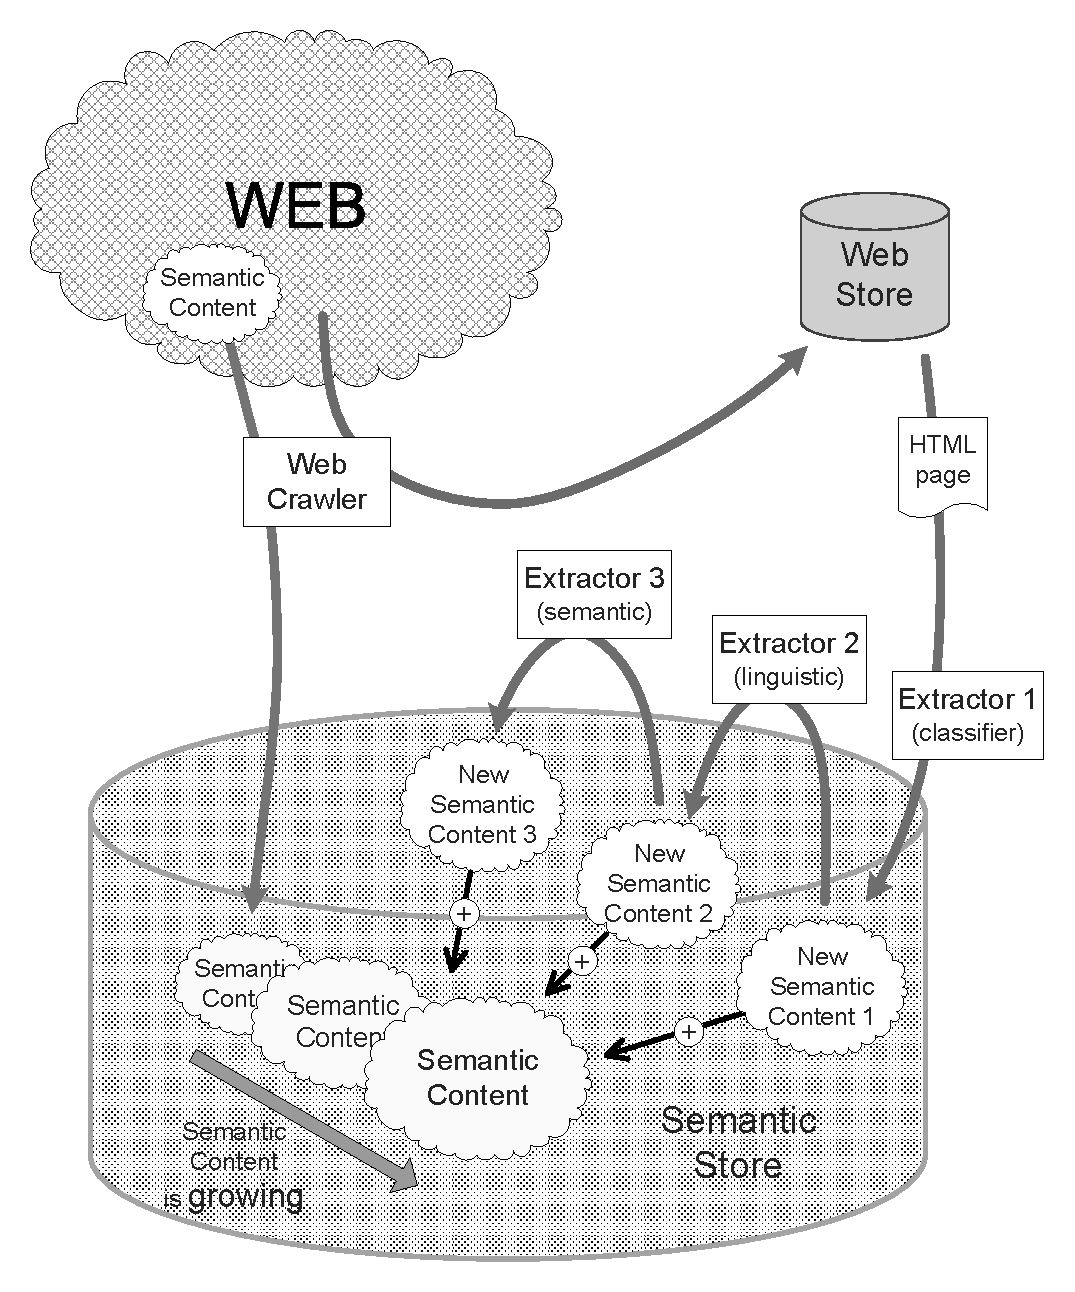
\epsfig{file=img/Semantization, height=\hsize, width=\hsize}
\caption{The process of semantization of the Web}
\label{img:Semantization}
\end{figure}


%\subsection{Motivation example}

%Our motivation example aims to illustrate a possible use of such a semantized web by an intelligent agent. Imagine a user wanting to buy a car. She has special requirements on car properties (possibly containing conflicting objectives as price and consumption) and its safety when used in Czech Republic (she knows about the increase of traffic accidents after unification of Germany, when fast western cars crashed on narrow roads of eastern part often \textbf{[6??]}).  Information about car properties can be extracted from several web shop pages typically in tables. Information about involvement in traffic accidents and if involved, then of injury rate, are hidden e.g. in textual traffic accidents reports of regional fire department (in Czech Republic responsible for emergency recovery). Our semantic store contains these information annotated (by possibly several tools) also by uncertainty of extraction and/or annotation process. Our intelligent agent can aggregate these (often conflicting) information and offer user best (top-k) answers according to a user dependent equilibrium between car properties, safety and reliability and/or (un)certainty of this information.

%\subsection{Our contributions}

%Our main contribution is the proof of concept of the idea of semantization of the web of today as an automated process making it ready for intelligent machine search. Particular contributions consists of models, methods and tools of :

%\begin{itemize}
%\item web repository based on highly efficient web crawler and a repository with extended soft computing classification (search) capabilities (see chapter 4??); 
%\item automated domain independent intermediate annotation of suitable pages from our web repository with soft computing heuristics (see chapter 5??);
%\item automated domain dependent annotation with extraction ontology and ILP learning from similar repeating structured linguistic data (see chapter 6??); 
%\item Semantic repository serving as a sample of semantized web, extension of the ontology model for additional annotation (e.g. uncertainty annotation) (see chapter 7??)
%\item Intelligent agent using soft computing tools for matching user preferences (see chapter 8??).
%\end{itemize}
%



%\section{Where is the problem with semantization of the Web of today?}

%Web of today contains lot of valuable information which is worth of being subject of intelligent search (also archived non-existing pages, e.g. http://www.archive.org/index.php and http://www.searchengineshowdown.com/others/archive.shtml ). Main obstacle is that these resources are designed for human consumption and are hardly understandable for a machine. The size of these resources excludes human search. Using traditional search engines has limited capabilities. One solution is to semantically enrich these pages (semantize) and make them machine processable.  As it is not an easy task, the problem is who will do it and why. This is well under way for new corporate applications and publishers willing to annotate their resources and the driver can be better services (and higher profit, faster emergency warning, ... \textbf{[3??]}).

%A step in direction of semantic enrichment is presented also by indexes of various search engines - they represent a certain sort of semantic enrichment. The problem is that those indexes are not available for writing own applications. Moreover search engines of today fail in linguistic search. Fixed page rank prohibits one to find relevant pages which are not highly quoted (e.g. traffic accident reports). Web shops enable only conjunctive query search. Web shops are mainly classified as hidden web, and are hard for machine processing. Survey pages can usually find cheapest item (when you know what you want). Linguistic search engines are just starting to be developed, mainly with some narrow focus. Another step to semantic enrichment are different WIE - 

%Web Information Extraction tools, nevertheless they do not annotate sources, From our point of view, we see the main problem of current tools with own enrichment of web content is that this enrichment mostly serves query answering and does not produce annotation of sources accessible for public for further processing.
%When we understand semantization (of the web of today) as a semantic enrichment automatically producing semantically annotated resources for further (third party) machine processing, then main problems of semantic enrichment of the web are:
%\\- How to do it automatically, in which order, which pages should be enriched first, \dots? Do the enrichment in the time of query or in advance?
%\\- Where to store such enriched (annotated) pages?
%\\- With respect to which ontology to make annotation?
%\\- What are metrics of satisfactory semantic enrichment?
%\\- When done, how to use it? Current RDF querying languages are not very promising for intelligent search.
%\\- How to achieve reusability/social web - agent once trained can be used by other user (with changed user preferences)
%\\- Which extractors are trustworthy; which URLs to search (Czech car offers)
%\\- User friendly - no need to search by keyword, only user preferences input.
%\\- Automation - when a new offer emerges on a page, extractor captures the information, stores it in the semantic store and agent has always information up-to-date.
%\\- When one extractor misses an attribute value, another can find it and store it. Such an automated semantic enrichment will be error prone. How to represent uncertainty? Problem of complete information?
%







\section{Idea of Web semantization}
%Here we would like to present the idea of our contribution to web semantization.

\textbf{First idea is the idea of a web repository.} In details it develops as follows. Semantic enrichment is in fact an inductive task (although a special one) - to add to web documents knowledge (which is obvious for human perception not for a machine). Such an inductive task will be easier to solve when there is a sort of repetition (modulo some similarity). So our initial idea is to use repetitions for our inductive task (which is to annotate data by concepts from an ontology which is the same as to map instances to ontology). 

Semantically enrich the web by an automated process is a time consuming task (not mentioning other problems) and hence only durable pages are worth to semantically annotate (so to say, before they are changed). 

Further restriction is to enrich only textual content, no multimedia (this substantially reduces size of information we have to store). Especially we restrict to pages with content consisting either dominantly of grammatical sentences (let us call them grammatical pages) and those containing large number of table cells (let us call them table pages). Of course this division need not be disjoint, and will not cover the whole web. 
To be able to separate durable grammatical or table pages with repetitions poses special requirements to search in our web repository.

\textbf{Second idea is to split annotation process to two parts}, one domain independent intermediate annotation and second domain dependent user directed annotation. Both should be automated, with some initial human assisted learning. This first part of learning could require assistance of a highly skilled system manager; the second (probably faster part) should be doable by an administrator with average computer literacy. 

\textbf{Domain independent intermediate annotation} can be done with respect to general ontologies. First ontology is the general PDT tectogrammatical structure which captures semantic meaning of a grammatical sentence (this is a task of computational linguistics; we make use of their achievements which were originally focused on machine translation). For structured survey pages we assume that their structure is not changing very often and many pages are generated by same tool, hence they are similar. So there is a chance to detect data regions and data records and possibly also attributes and values from detailed product pages. Here annotation tools will be also trained by humans -- nevertheless only once for the annotation of the whole repository. 

\textbf{Domain (task) dependent (on demand) annotation} is concerning only pages previously annotated by general ontologies. This makes second annotation faster and easier. Here an assistance of a human is assumed for each domain and new ontology. For grammatical pages repetitions make possible to learn mapping from structured tectogrammatical instances to an ontology. For structured pages the annotation tool has to learn some form of extraction ontology. This domain (task) dependent task can be avoided by a collaborative filtering method, assuming there is enough users' acquaintance. In the future, the second should be doable by an administrator with average computer literacy. 

Further important idea is do \textbf{design semantic repository}. Besides above mentioned annotations it should contain some sort of uncertainty annotation. The main reason is that annotation process is error prone and we can have in future different alternative annotation tools and aggregate results. 

Last, but most \textbf{important idea is to design at least one agent} which will give evidence that our semantization really improved general web search. Besides using annotated data it should also contain some user dependent preference search capabilities

 
The process of a user searching for a used car is represented in Figure 2??. Our main focus is in the agent and in the extractors. 

Last idea is to use soft computing techniques, because the whole problem is too hard to be solved by crisp techniques. 


\section{Egothor support for web repository}
Egothor allows an easier retrieval of Web documents stored in the Web repository for the semantic extractors. Some functionality will be described together with the proposal of parts of our system, especially agent (Sections 5-8???). This section describes in detail and explains how Egothor runs and supports the Semantic Search engine.

\subsection{Crawler}

Egothor crawler is designed for high-speed efficient Web crawling. The software was implemented in Java with a strict use of NIO operations. This technology ensures high throughput (up to several MB per second on a single node) and minimizes a number of crawler fetch threads (in Figure 3 yellow parts are outside of Egothor, green filters are emphasized because of their role in our application).
 
The central component of the crawler is a scheduler. It prepares a plan of URLs which are (re)crawled next.  The plan is affected by many factors stored in crawler's knowledge-base: network link quality, website size, number of HTTP errors during the communication with a website, history of changes in website documents in past, and other minor attributes. The knowledge-base allows the crawler to act promptly if anything (may) slow him down.

The plan is executed by a fetch thread and then the crawled documents enter a parser. The parser is responsible to extract a next fragment of a link structure and new URLs. It also prepares SAX stream which is later analyzed by an acyclic net of filters. Each of the filters may add new tags (labels on a document) and modify the SAX stream for successive filters. The output of the filtering machinery is processed by a full-text indexer and stored in an auxiliary buffer (index chunk).  The index chunks are merged with a main index using a dynamization algorithm. Original Web documents, including the tags added by the filters, are stored in the Web repository.

The filters must operate on the SAX stream only and cannot use any context information (who points to this page, what pages are similar, etc.) due to performance reasons. Therefore, they are able to provide a simple classification by tags like: page with HTML FRAMEs, TABLEs, real grammatical sentences (if the filter can find reasonable punctuation).


\subsection{Web repository}
The Egothor repository is a temporal repository of Web documents; therefore a document is identified by its id, revision number and a timestamp. The documents come together with their initial tags, and these tags can be freely modified later. The tags simplify a retrieval of documents, since you can use them instead of raw document ids and revision numbers. Moreover, the repository is also able to retrieve documents where a given Boolean formula of tags matches. The repository recognizes two tag groups: some tags are read as "for all revisions of a concrete document", while others are tied with just a given document revision.

The architecture is based on three layers: core that saves documents and computes deltas between revisions to save space; symlink that maps core's document and revision numbers to numbers published to a user; cloud that assigns tags and manages ACL on the tags. This way the system can modify the tags without overloading the main base of raw documents.

The repository supports document's metadata, e.g. modification and creation dates. It keeps track of all changes in a document, so that it is able to provide information about a durable (persistent) text blocks or even subtrees in DOM.





\section{Intermediate domain independent automated annotation}
Web information extraction is often able to extract valuable data. We would like to couple this process with consecutive semantic annotation (initially human trained; later it should operate automatically). In this chapter we would like to describe details of our idea to split this process in two parts - domain independent and domain dependent. There are several reasons of this. 

The first domain independent annotation will serve as an intermediate annotation supporting further processing. This will run once on whole suitable data. Hence necessary human initial assistance by training can be done by a high skilled expert (indeed it can be a long process).
The second domain dependent annotation part can consists of large number of tasks with different domains and ontologies. This should be possible to train very fast and if possible with assistance of an average computer skilled administrator. Having intermediate annotation we can afford this. 

We have identified two types of web resources where this can be done. First are "table pages", containing large number of cells with abbreviated description of a resource and corresponding detailed pages. Here we assume that content of cells is similar and content of detailed pages is also similar. Second are pages dominantly consisting of grammatical sentences. Thanks the fact that we have a third party linguistic tool for creation of tectogrammatical trees of sentences, this can be done without requirement of similarity repetition. This situation is illustrated in the Table 1.


\begin{table}
{\tiny\begin{tabular}{|c|c|c|} \hline
Type of annotation&Table pages&Grammatical pages\\ \hline
Intermediate general&Uses similarities&Does not use similarities\\ \hline
Domain dependent&Does not use similarities&Uses similarities\\ \hline
\end{tabular}}
\label{table1}
\caption{Use of similarity in annotation approaches}
\end{table} 

\subsection{Structural similarity extraction tool}
First approach for domain independent intermediate information extraction and semantic annotation is to use the structural similarity in web pages containing large number of table cells and for each cell a link to detailed pages. This is often presented in web shops and on pages that presents more than one object (car). Each car is presented in a similar way and this fact can be exploited.

As web pages of web shops are intended for human usage creators have to make their comprehension easier. Acquaintance with several years of web shops has converged to a more or less similar design fashion. There are often cumulative pages with many products in a form of a table with cells and some brief description and then there are links detailed pages to each product. Of course many pages of Web shops belong to hidden (deep) web and require some form of initialization. Links to detailed pages can be replaced by some scripts. This can make the crawling of such pages problematic; we do not solve this problem here. Once (a part of these pages) is crawled and stored in our Egothor repository, we can process them further. 

Main idea (illustrated in the Figure 4???) is to use a DOM tree representation of the summary web page and by breadth first search encounter similar subtrees. The similarity of these subtrees is used to determine the data region - a place where all the objects are stored. It is represented as a node in the DOM tree, underneath it there are the similar sub-trees, which are called data records. Our ontology engineering part is based on a bottom-up approach of building ontologies. The first classes are "table page", "data region" and "data record" which are connected with properties "hasDataRegion" and "hasDataRecord". Also, between data record and its detail Data\_region and Detailed\_page we have property "hasDetailPage". Note that these concepts and properties have soft computing nature which can be modeled by a fuzzy ontology. For instance, being an instance has a degree of membership depending on the precision of our algorithm (dependent on similarity measures used to detect data regions and/or records). Using some heuristics we can detect what are resources described in this page (Table\_page describes rdfs:Resources). To detect possible attributes and even their values we explore similarities between data record content and corresponding detailed page content. The main idea is to find same pieces of text in the data record and in the detail page. This occurs often, because a brief summary of the object is present in the data record. Somewhere near the attribute values are located the names of attributes in the detail page. These names of attributes can be extracted. The extraction of attribute names is easy because on every detail page the names will be the same.  The names of attributes can be used in our low-level ontology as names of properties - each object will be represented by the URL of the detail page, and a set of properties that consists of the attribute values found on the detail page.

This idea was implemented in [5???] on the top of Mozilla Firefox API and experimentally tested on table pages from several domains (cars, notebooks, hotels). Tree representation was the DOM of the page, similarity between subtrees was Levenshtein editing distance (for a subtree considered as a linear string), learning thresholds for decision were trained (more see [13???]).

\begin{figure}
{\footnotesize\begin{verbatim}
1 function BFSfindDR(LevelNodes)
2 begin
3   NextLevelNodes =  ; 
4   regions =  ; 
5   for each Node in LevelNodes do 
6   begin 
7     regions=identDataRegions(normalized(Node.children)); 
8     NextLevelNodes=NextLevelNodes  U 
	      (Node.Children not in regions);         
9   end
10    if NextLevelNodes !=   
11      return regions U BFDfindDR(NextLevelNodes);
12    else return regions;
13 end
\end{verbatim}}
\caption{Algorithm for finding data regions on a web page}
\label{fig:alg}
\end{figure}

Input of algorithm in Figure~\ref{fig:alg} is the root element of the DOM tree of a web page. Function BFSfindDR is recursive; each run processes one tree level. Algorithm proceeds across each node of input LevelNodes (5) and tries to identify if some of the node's children represent a data regions (7). If so, those children are excluded from further processing (8). Nodes that are not in data regions are added to NextLevelNodes. Finally, if there are some nodes in NextLevelNodes, the function is called recursively. Data regions found on the page form the output of function.
Further improvement of annotation is left for domain dependent annotation where special extraction ontology can be trained (e.g. containing regular expressions for this special domain).

\subsection{Method based on Czech linguistics}
Second approach for Web information extraction is based on Czech linguistics and NLP tools. We use a chain of linguistic analyzers (\cite{biblio:HajicMorfTag}, \cite{biblio:collinshbrt_1999}, \cite{biblio:KlTransformationBasedTectogrammatical2006}) that process text presented on a web page and produce linguistic (syntactic) trees corresponding with particular sentences. These trees serve as a basis of our semantic extraction.

Unlike the usual approaches to the description of English syntax, the Czech syntactic descriptions are dependency-based, which means, that every edge of a syntactic tree captures the relation of dependency between a governor and its dependent node. Especially the tectogrammatical (deep syntactic) level of representation \cite{biblio:MiBeAnnotationtectogrammatical2006} is closer to the meaning of the sentence. The tectogrammatical trees (Example of such a tree will be presented in section 6.3??? on the Figure 8???) have a very convenient property of containing just the type of information we need for our purpose (extraction of semantic information), namely the information about inner participants of verbs - actor, patient, addressee etc. So far this tool does not work with the context of the sentence and hence does not exploit frequent occurrence of similar sentences.





\section{Domain dependent automated annotation}
Second phase of our extraction-annotation process is domain dependent. It can make use of previous intermediate general (domain independent) annotation. Our goal is to make this process fast and as easy as possible, e.g. to be trained by an average computer skilled administrator very fast and precise. As in previous cases, also here several aspects need soft computing heuristics and can be recorded in an ontology.

\subsection{Extraction and annotation based on extraction ontology}
Domain ontology (on the Figure 6???) is the basis for extraction ontology. Extraction ontology [19???] extends the domain ontology by adding some additional information about how the instances of a class are presented on web pages. We used regular expressions for some of the properties of class \emph{CarType}. These regular expressions are matched against the text found on the web page. 

So far the creation of extraction ontology has to be done by a very experienced user and has to be verified on a set of web pages. In the future we plan to invest more effort and soft computing techniques in automating this part.

In this paper we do not deal with learning of extraction ontology. Please notice, that parts of domain ontology are properties \emph{ratioOfAccidents} and \emph{ratioOfDeath}, which have cumulative values obtained from linguistic extraction over the whole corpus. 

\subsection{Domain dependent Extraction and annotation based on linguistics}

Assume we have pages annotated by linguistic annotator and we have a domain ontology. The extraction method we have used is based on extraction rules. An example of such extraction rule is on the Figure 7??? (on the left side). These rules represent common structural patterns that occur in sentences (more precisely in corresponding trees) with the same or similar meaning. Mapping of the extraction rules to the concepts of target ontology enables the semantic extraction. Example of such mapping is demonstrated in the Figure 7???.

We experimented with obtaining extraction rules in two ways.
\begin{enumerate}
\item Rules and mappings were designed manually (like the rule on the Fig. 7???) and 
\item rules and mappings were learned using Inductive Logic Programming (ILP) methods (see following section).
\end{enumerate}


\subsection{Using Inductive Logic Programming (ILP)}
ILP is a method for generation of rules that describes some properties of data. It takes three kinds of input
\begin{itemize}
	\item Positive examples E+ -- objects that have the desired property.
	\item Negative examples E- -- objects that do not have the desired property.
	\item Background knowledge -- facts about the domain (so far we do not consider background knowledge in the form of rules).
\end{itemize}

ILP tries to generate such rules that all positive examples and no negative example satisfy them. It uses concepts from the background knowledge in the body of rules.
The main advantage of ILP is that it can be trained to mine arbitrary data described in predicate logic - the process of learning is dependent only on the positive and negative examples and on the amount of information we have about them. The more information we have, the more precise the learning will be. 

Thanks to the fact that ILP learns from positive and negative examples, we can propose an assisted learning procedure for learning and also tuning the extractor (described in previous section). The process is such that extractor gets pure textual or semantically annotated (by the extractor) data from a web page and presents it to the user. He or she then annotates or only corrects the data saying which are good and which are badly annotated. Extractor can be learned and tuned to the desired goal in this way. Of course the user has to understand the semantics of the annotations - so he or she has to be an expert in that way of understanding the target ontology, but this ontology can be quite simple in the case we are interested only in a specific kind of information e.g. number of people injured during a car accident like in our experiments (see next section) and motivation. 

We discovered that we can use a straightforward transformation of linguistic trees (see an example on the Figure 8???) to predicates of ILP (example of the transformation is in the Figure 9???) and the learning procedure responds with significant results, which are presented in next section.

On the Figure 8??? we can see the relationship between particular words of a sentence and nodes of tectogrammatical tree -- the highlighted node of the tree corresponds with the word "two" in the sentence (also highlighted). This relationship allows propagation of information form user (which annotates just text of sentence) to the ILP learning procedure.


\subsection{Experiments}
Our experiment was to enable our agent to access information from various sources. The first source is data structured into tables, from which the semantic information is extracted. We used extraction tool [5???] for the extraction. Data extracted in this way represents car offers with attributes of the car offered, the price, the seller of the car etc.

In Table 2 is presented a typical form of extracted data (using the extraction tool [5???]). Data can be stored in a relational database or in an ontology as was described in Section 5.1??? and 6.1???. This data provide a base set of attributes that can be enriched by other source of data, for example from natural language texts.
The price of the car is in Czech crowns; about 17 Czech crowns is 1\$. There were more than one offer for each car type, we chose the offer randomly. In reality, all offers are stored in the ontology (as was presented in Figure 6???).

The second source of data is natural language text. We wanted to find out the number of injured persons during car accidents. We have used firemen reports; some of them were about car accidents, some were not. Each report was split into sentences and each sentence was linguistically analyzed and transformed into a tectogrammatical tree, as described in previous two sections. These trees were transformed to a set of Prolog facts (see Figure 9???). 
Sentences, which talk about an injury during a car accident, were manually tagged by predicate injured(X), where X is the ID of the sentence. Those sentences that do not talk about injured persons during a car accident were tagged as :-injured(X), which represents negative example. This tagging can be done even by an user unexperienced in linguistics and ILP, but he or she has to understand the semantics of information he is tagging (in usually means that he or she has to understand the target ontology).
These tagged sentences were input for ILP, we used 22 sentences as positive examples and 13 as negative examples. We used Progol [20???] as ILP software.
The rules ILP found are in following Table 3???.

\begin{verbatim}
injured(A) :- id(B,A), id(B,t_plzensky57770_txt_001_p5s2).
injured(A) :- id(B,A), id(B,t_plzensky60375_txt_001_p1s6).
injured(A) :- id(B,A), id(B,t_plzensky57870_txt_001_p8s2).
injured(A) :- id(B,A), id(B,t_plzensky57870_txt_001_p1s1).
injured(A) :- id(B,A), edge(B,C), edge(C,D), t_lemma(D,zranit).
injured(A) :- id(B,A), edge(B,C), edge(C,D), t_lemma(D,nehoda).
Table 3: Rules found by ILP
\end{verbatim}

The first four rules are overfitted to specific sentences. Only the last two represent generally applicable rules. But they do make sense - "zranit" means "to hurt" and "nehoda" means "an accident" in Czech. These two rules mean that the root element is connected either to a noun that means an accident or to a verb that means to hurt.
We tested these rules on the set of 15 positive and 23 negative examples. The result accuracy was 86.84\%. Results are in Table 4. P is the positive sentence from ILP, ~P is negative sentence, A is sentence tagged as positive and $\neg$A is sentence tagged as negative. 11 sentences that were tagged as positive were also tagged as positive by ILP, 4 was tagged as negative by ILP. 22 sentences that were tagged as negative were also tagged as negative by ILP, only 1 was tagged as positive by ILP.


\begin{verbatim}
	A	~A
P	11	1
~P	4	22
Table 4. Results on the test set.
\end{verbatim}


In this case we learned set of rules that identify relevant sentences - roots of relevant tectogrammatical trees. We understand these results as proof of concept that ILP can be also used for finding other kinds of information present in nodes and structure of linguistic trees. Se we can for example extract number of injured people from relevant trees if we modify the training data. 
The information extracted in this way can be combined with the information extracted from structured tables. If we extracted the information about the model of the car involved in the accident, we may count the number of accidents about each model; which may be valuable for the user when deciding about particular models of cars. 



\section{Conclusions and further work}
In this paper we have developed the idea of web semantization, which can help to arch over the gap between Web of today and the Semantic Web. We have presented a proof of concept that even today it is possible to develop a semantic search engine in the scale of *.cz pages and an intelligent software agent. In particular contributions consists of models, methods and tools of a web repository, two sorts of automated third party annotation of existing web resources, semantic repository serving as a sample of semantized web with extension of the ontology model for additional annotation (e.g. uncertainty annotation) and a proposal of an intelligent agent . In many places of this work, both in the modeling part and in implementation we have made use of soft computing techniques. 

Future work goes in two directions. First in integration of specific parts of the system,  in automation of the whole process and extensive experiments with larger number of different users. Second in improving special parts of the system -- either making it more precise or making it more automatic (able to train by a less qualified user).

%ACKNOWLEDGMENTS are optional
\section{Acknowledgments}
This work was partially supported by Czech projects \\1ET100300517, 1ET100300419 and MSM-0021620838.
%
% The following two commands are all you need in the
% initial runs of your .tex file to
% produce the bibliography for the citations in your paper.
\bibliographystyle{abbrv}
\bibliography{SWA_webSemantization}  % sigproc.bib is the name of the Bibliography in this case
% You must have a proper ".bib" file
%  and remember to run:
% latex bibtex latex latex
% to resolve all references
%
% ACM needs 'a single self-contained file'!
%
%\subsection{References}
%Generated by bibtex from your ~.bib file.  Run latex,
%then bibtex, then latex twice (to resolve references)
%to create the ~.bbl file.  Insert that ~.bbl file into
%the .tex source file and comment out
%the command \texttt{{\char'134}thebibliography}.
\balancecolumns % GM July 2000
% That's all folks!
\end{document}
